
\section*{Truncated gamma distribution}

Consider the $P_{ij}$ to follow the continuous \textbf{truncated gamma distribution}, which is given by the density function $f^T$ as
\begin{align}
  f_{\alpha,\beta}^T(x) = \begin{cases} K_{\alpha, \beta}\,
\frac{1}{\beta^{\alpha}\Gamma(\alpha)}\, x^{\alpha-1}\,e^{-x/\beta} & 0 \leq x \leq 1 \\
0 & \text{otherwise},
\end{cases}
\end{align}

where the normalization factor $K_{\alpha,\beta}$ is the inverse of the cumulative
probability that $x \leq 1$ of the untruncated gamma distribution 
\begin{align}
  K_{\alpha,\beta} = \left(\int_0^{1} \frac{1}{\beta^{\alpha}\Gamma(\alpha)}\, x^{\alpha-1}\,e^{-x/\beta} \, dx \right)^{-1}.
\end{align}
When the overall connection probability $\mu$ is fixed, only one free parameter remains, and the relative overrepresentation of bidirectional connections $\varrho$ can be approximated as
\begin{align}
 \varrho \approx  1 + \frac{1}{\alpha}.
\end{align}

\begin{center}\vspace{1cm}
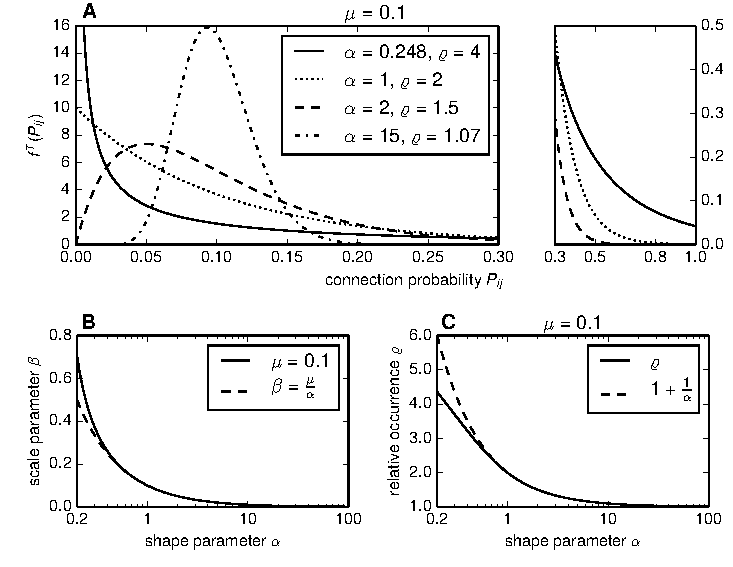
\includegraphics[width=0.9\linewidth]{gamma_figure.pdf}
\captionof{figure}{ \textbf{A} Probability density functions of the
  truncated gamma distribution for different shape parameters $\alpha$
  and the induced relative overrepresentation $\varrho$ in the network
  with such distributed connection probabilities $P_{ij}$. For a given
  $\alpha$, the scale parameter $\beta$ was chosen such that $\mu =
  0.1$. \textbf{B} Contour of $\alpha$, $\beta$ pairings
  that yield an overall connection probability of $\mu =
  0.1$. \textbf{C} Relative occurrence $\varrho$ in dependence on
  $\alpha$ for fixed $\mu = 0.1$. For $\alpha \geq 1$ this
  relationship is well approximated by $\varrho \approx 1 +
  \frac{1}{\alpha}$.}
\end{center}\vspace{1cm}
